\documentclass[12pt,fleqn]{article}
\setlength{\parindent}{0pt}
\usepackage{graphicx}
\usepackage{cancel}
\usepackage{listings}
\usepackage[latin5]{inputenc}
\setlength{\parskip}{8pt}
\setlength{\parsep}{0pt}
\setlength{\headsep}{0pt}
\setlength{\topskip}{0pt}
\setlength{\topmargin}{0pt}
\setlength{\topsep}{0pt}
\setlength{\partopsep}{0pt}
\setlength{\mathindent}{0cm}

\begin{document}
Entegralleri Nasil Dusunelim

Calculus kitaplarinda entegralleri anlatmak icin cogu zaman ``toplam''
kavrami on plana cikarilir, mesela alttaki resimde $f(x)$ fonksiyonunun
altinda kalan ufak ufak dikdortgenlerinin alanlarinin toplamindan
bahsedilir. 

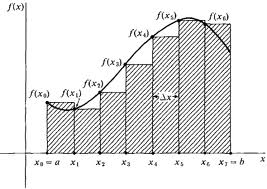
\includegraphics[height=4cm]{area.png}
Fakat bu tur bir anlatim bazen karisikliga yol acabiliyor. Daha iyi bir
anlatim entegralin ``degisen degerlerin carpimi'' oldugudur. Alttaki
resimdeki dikdortgeni dusunelim, 

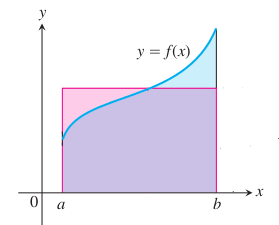
\includegraphics[height=4cm]{box.png}
ve bu dikdortgen entegralin hesapladigi alani yaklasiksal olarak
hesapladigini farzedelim. Dikdortgen alani nasil hesaplanir? Iki kenarinin
carpilmasiyla! Entegral de aslinda boyle bir hesaptir, sadece kenarlardan
biri sabit degildir, ve surekli degismektedir. Bu tur bir anlayis birimleri
sonuca dahil etmek gerektiginde ise yarar, mesela yatay eksen $t$ ise, ve
dikey eksen $v(t)$ yani hiz ise, katedilen mesafe, $v(t)$ nasil bir sekilde
olursa olsun, 

\[ \int v(t)dt \]

ile hesaplanacaktir. 















\end{document}
